\chapter{自由基、卡宾与重排}\label{ch:b3:radicals-carbenes}

除虫菊以菊酸的酯类自我防御，这些分子以
三元碳环为骨架；其合成类似物是最常用的
家用杀虫剂之一。化学家一步闭合此类环，方法是
向双键加成\omterm{def:b3:organometallic-bonding:carbene}{卡宾}：\omterm{def:b3:organometallic-bonding:carbene}{卡宾}是碳原子，周围只有六个电子，
其中两个未成键。本章讨论活性中间体，它们在
本科一年级与二年级分册中仅略有涉及（用于合成的自由基、
\omterm{def:b3:organometallic-bonding:carbene}{卡宾}和\omterm{def:b3:radicals-carbenes:nitrene}{氮宾}），还讨论一类重排反应，其中某一基团
迁移至缺电子的碳、氮或氧原子上，其中两例
所得产物分别是尼龙-6 和一种可生物降解聚酯的单体，二者
出自同一种酮。

\begin{recall}
本科一年级分册介绍了自由基、均裂和单钩箭头，
碳正离子及其重排、亲核试剂与离去基团；
本科二年级分册介绍了自由基\omterm{def:b3:complex-kinetics:chain}{链反应}（链引发、链增长、链终止、
自由基引发剂）、过氧酸、内酯、内酰胺和亚胺。
\Cref{ch:b3:complex-kinetics}讨论了\omterm{def:b3:complex-kinetics:chain}{链反应}动力学，
\cref{ch:b3:organometallic-bonding}讨论了作为配体的\omterm{def:b3:organometallic-bonding:carbene}{卡宾}，
\cref{ch:b3:many-electron-atoms}讨论了\omterm{def:b3:many-electron-atoms:singlet-triplet}{单重态}与\omterm{def:b3:many-electron-atoms:singlet-triplet}{三重态}，以及
\cref{ch:b3:rate-theories}讨论了哈蒙德假设。
\end{recall}

\begin{omfigure}
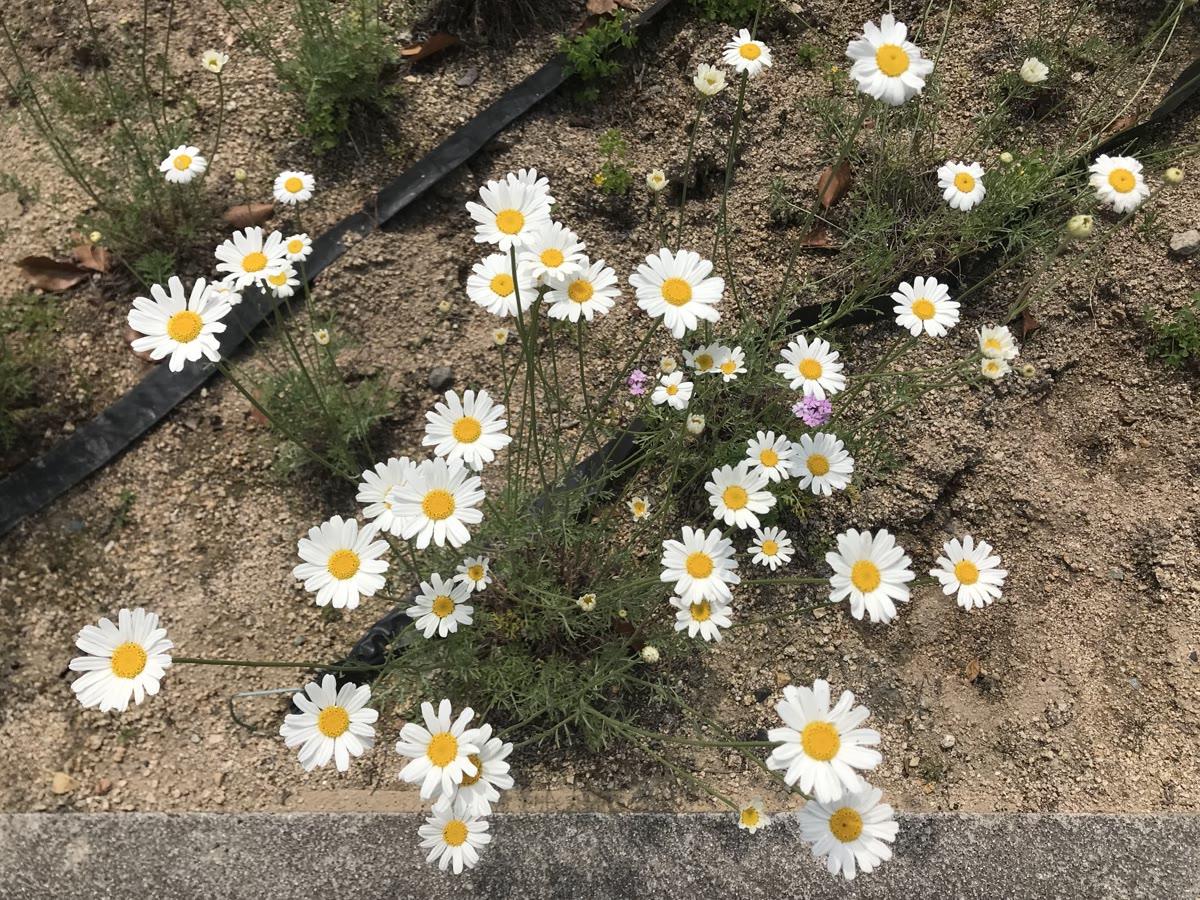
\includegraphics[width=0.48\linewidth]{images/book4/pyrethrum.jpg}

{\small 除虫菊。其花中含有除虫菊素，即一类杀虫的
环丙烷羧酸酯类。摄影：Soramimi，CC BY-SA 4.0。}
\end{omfigure}

\section{合成中的自由基链反应}

碳自由基的稳定性，可由生成它的 C--H 键的
键解离焓来衡量：键越弱，自由基就越
稳定。

\begin{proposition}[键解离焓]\label{prop:b3:radicals-carbenes:bde}
在\qty{298}{K}下，R--H 键的键解离焓由气相
生成焓求得：$\mathrm{BDE(R{-}H)} = \Delta_fH^\circ(\mathrm R^\bullet) + \Delta_fH^\circ(\mathrm H^\bullet) - \Delta_fH^\circ(\mathrm{RH})$。
\end{proposition}

\begin{proof}
由盖斯定律，均裂 $\mathrm{RH \to R^\bullet + H^\bullet}$ 的反应焓
等于生成物生成焓之和减去反应物的生成焓；该反应焓即
为键解离焓（按定义）。
\end{proof}

\begin{omfigure}
% ledger: dfh4:CH3r, dfh4:C2H5r, dfh4:iC3H7r, dfh4:tC4H9r, dfh4:PhCH2r, dfh4:H, dfh:CH4_g, dfh:C2H6_g, dfh:C3H8_g, dfh4:iC4H10, dfh4:toluene_g
\begin{tikzpicture}
\begin{axis}[width=0.72\linewidth, height=5.2cm, ybar, bar width=16pt, ymin=350, ymax=450,
  xtick={1,2,3,4,5}, xticklabels={{$\ce{CH3-H}$}, {$\ce{C2H5-H}$}, {$\mathrm{(CH_3)_2CH{-}H}$}, {$\mathrm{(CH_3)_3C{-}H}$}, {$\ce{C6H5CH2-H}$}},
  x tick label style={font=\scriptsize}, ylabel={键解离焓 / \unit{kJ.mol^{-1}}},
  axis lines=left, tick label style={font=\scriptsize}, label style={font=\small},
  nodes near coords, nodes near coords style={font=\scriptsize, /pgf/number format/fixed, /pgf/number format/precision=0},
  enlarge x limits=0.15]
\addplot[fill=omDef!55, draw=omDef] table[x=i, y=bde] {figdata/out/bachelor-3-bde.dat};
\end{axis}
\end{tikzpicture}

{\small C--H 键在\qty{298}{K}下的键解离焓，由气相
分子与自由基的生成焓计算得到：甲基、伯、
仲、叔和苄基 C--H 键。所生成的自由基取代程度越高，
或共轭程度越大，该键越弱。}
\end{omfigure}

\begin{proposition}[卤代反应的选择性]\label{prop:b3:radicals-carbenes:halogenation-selectivity}
溴原子夺氢时，在伯、
仲、叔 C--H 键之间的选择性远高于氯原子夺氢。
\end{proposition}

\begin{proof}[论证]
由于 $\mathrm{BDE(H{-}Cl)}$ 大于图中所有 C--H 值，而 $\mathrm{BDE(H{-}Br)}$ 更小，
氯原子夺氢为放热，溴原子夺氢为吸热。由哈蒙德
假设（\cref{ch:b3:rate-theories}）可知，氯的过渡态较早、
类似反应物，几乎不感受所生成自由基间的差别；
溴的过渡态则较晚、类似产物，其活化能大部分
随 BDE 之差而变化，玻尔兹曼因子将之转化为很大的速率比。
\end{proof}

三丁基氢化锡借\omterm{def:b3:complex-kinetics:chain}{链反应}还原卤代烷：锡自由基夺取
卤原子，烷基自由基则从下一分子的氢化锡上夺取
氢原子，并生成新的锡自由基。同一\omterm{def:b3:complex-kinetics:chain}{链反应}还可去除羟基
一旦将其转化为硫代羰基酯（巴顿–麦康比
脱氧反应），并可闭环。有机锡残留有毒，且难以
去除；三（三甲基硅基）硅烷及其他硅烷，如今常取代
氢化锡。

\begin{omfigure}
\begin{tikzpicture}[font=\small, >=Stealth]
  \node (a) at (-2.0,0) {$\mathrm{Bu_3Sn^\bullet}$};
  \node (b) at (2.0,0) {$\mathrm{R^\bullet}$};
  \draw[->, thick] (a) to[bend left=35] node[midway, above, font=\scriptsize] {$+\,$R--Br, $\ -\,\mathrm{Bu_3SnBr}$} (b);
  \draw[->, thick] (b) to[bend left=35] node[midway, below, font=\scriptsize] {$+\,\mathrm{Bu_3SnH}$, $\ -\,$R--H} (a);
  \node[font=\scriptsize, align=center, anchor=north] at (0,-1.5) {链引发：AIBN $\xrightarrow{\Delta}$ 2 R$'^\bullet$ $+$ $\ce{N2}$; \ R$'^\bullet$ $+$ $\mathrm{Bu_3SnH}$ $\to$ R$'$H $+$ $\mathrm{Bu_3Sn^\bullet}$};
\end{tikzpicture}

{\small 氢化锡还原溴代烷的链增长步骤。
每还原一个 R--Br 消耗一分子 $\mathrm{Bu_3SnH}$，生成一分子 $\mathrm{Bu_3SnBr}$；\omterm{def:b3:complex-kinetics:chain}{链载体}
为锡自由基和烷基自由基。}
\end{omfigure}

溴化氢在过氧化物存在时，以同类\omterm{def:b3:complex-kinetics:chain}{链反应}加成到烯烃上，
溴原子加成到取代程度较低的一端，生成
更稳定的自由基，随后从 HBr 夺取一个氢原子：
反马氏加成。

\section{自由基环化}

\begin{definition}[外型环化与内型环化]\label{def:b3:radicals-carbenes:cyclisation}
在\emph{外型环化}\index{外型环化}中，被断裂的键（或
被进攻的 $\pi$ 键）位于新环之外；在\emph{内型环化}\index{内型环化}
中则位于新环之内。
\end{definition}

\begin{omfigure}
\begin{tikzpicture}[font=\scriptsize, >=Stealth]
  % hex-5-enyl radical: C1 radical, C5=C6
  \foreach \i/\a in {1/162, 2/234, 3/306, 4/18} { \coordinate (p\i) at (\a:0.9); }
  \coordinate (p5) at (90:0.95); \coordinate (p6) at (90:1.9);
  \draw[thick] (p1) -- (p2) -- (p3) -- (p4) -- (p5);
  \draw[thick, double, double distance=1.5pt] (p5) -- (p6);
  \node[anchor=east] at (p1) {$\bullet$\,1};
  \node[anchor=west] at (p5) {5}; \node[anchor=west] at (p6) {6};
  \draw[->, omMeth, thick] ($(p1)+(0.1,0.15)$) to[bend left=25] node[pos=0.45, below right, inner sep=1pt] {5-外型} ($(p5)+(-0.15,-0.05)$);
  \draw[->, omThm, thick, densely dashed] ($(p1)+(0,0.25)$) to[bend left=50] node[midway, left] {6-内型} ($(p6)+(-0.2,0)$);
  \node[font=\small, align=center] at (0,-1.6) {己-5-烯基自由基};
  \draw[->, thick] (1.6,0.3) -- (2.7,0.3) node[midway, above] {快};
  \begin{scope}[xshift=4.0cm]
    \foreach \i/\a in {1/162, 2/234, 3/306, 4/18, 5/90} { \coordinate (q\i) at (\a:0.75); }
    \draw[thick] (q1) -- (q2) -- (q3) -- (q4) -- (q5) -- (q1);
    \draw[thick] (q5) -- ++(90:0.6) coordinate (q6);
    \node[anchor=south, inner sep=1pt] at (q6) {$\mathrm{{}^\bullet CH_2}$};
    \node[font=\small, align=center] at (0,-1.6) {环戊基甲基自由基};
  \end{scope}
\end{tikzpicture}

{\small 己-5-烯基自由基通过 C1 进攻 C5 而闭环（5-外型，绿色）：
新环含五个成员，自由基位于环外的 C6 上。进攻 C6
（6-内型，红色虚线）会生成更稳定的仲环己基自由基，
但速率慢得多：链无法使 C1 处于
$\pi^*$ 轨道所要求的、接近 C6 的进攻方向上。}
\end{omfigure}

\begin{proposition}[鲍德温规则]\label{prop:b3:radicals-carbenes:baldwin}
对于成环（经实验确立，并有立体电子学依据）：
在四面体碳（tet）上，3 至 7 元\omterm{def:b3:radicals-carbenes:cyclisation}{外型环化}有利，5、6 元\omterm{def:b3:radicals-carbenes:cyclisation}{内型环化}不利；
在三角碳（trig）上，3 至 7 元\omterm{def:b3:radicals-carbenes:cyclisation}{外型环化}有利，3 至 5 元\omterm{def:b3:radicals-carbenes:cyclisation}{内型环化}不利，
6、7 元\omterm{def:b3:radicals-carbenes:cyclisation}{内型环化}有利；在二角碳（dig）上，3、4 元\omterm{def:b3:radicals-carbenes:cyclisation}{外型环化}不利，
5 至 7 元\omterm{def:b3:radicals-carbenes:cyclisation}{外型环化}有利，3 至 7 元\omterm{def:b3:radicals-carbenes:cyclisation}{内型环化}有利。
\end{proposition}

这一规则的依据是各类键所需的进攻角度：在四面体碳上，须从键的背面
以约 107° 的角度进攻；对三角 $\pi$ 体系，
所需角度较小；对三键则更窄。短链无法到达
这些位置，因此上述不利的情形无法实现。

\begin{definition}[自由基钟]\label{def:b3:radicals-carbenes:radical-clock}
\emph{自由基钟}\index{自由基钟}是一种自由基，它会以已知速率常数发生单分子重排，
如己-5-烯基自由基的环化；
它与双分子捕获剂的竞争可用来测定
捕获剂的速率常数，或反之。
\end{definition}

\begin{proposition}[竞争动力学]\label{prop:b3:radicals-carbenes:clock}
若自由基或发生环化（$k_c$），或被过量存在的氢化物捕获，
该氢化物浓度为 $[\mathrm{R_3SnH}]$（$k_H$），则产物比为
$[\text{环化}]/[\text{直接}] = k_c/(k_H[\mathrm{R_3SnH}])$。
\end{proposition}

\begin{proof}
任一时刻，两种产物的生成速率分别为 $k_c[\mathrm R^\bullet]$ 与 $k_H[\mathrm{R_3SnH}][\mathrm R^\bullet]$。其比值
不依赖于自由基浓度（自由基浓度是变化的）；在氢化物浓度恒定时，
对时间积分会使两者乘以同一因子
$\int[\mathrm R^\bullet]\,\dd t$，于是产物之比等于速率常数之比
乘以 $1/[\mathrm{R_3SnH}]$。
\end{proof}

\begin{omfigure}
\begin{tikzpicture}
\begin{axis}[name=a, width=0.47\linewidth, height=5.2cm, xmode=log, xmin=1e-3, xmax=1, ymin=0, ymax=1,
  axis lines=left, xlabel={$[\mathrm{Bu_3SnH}]$ / \unit{mol.L^{-1}}}, ylabel={环化分数},
  tick label style={font=\scriptsize}, label style={font=\small}]
\addplot[omDef, thick] table[x=c, y=fcyc] {figdata/out/bachelor-3-radical-clock.dat};
\end{axis}
\begin{axis}[at={(a.east)}, anchor=west, xshift=1.5cm, width=0.47\linewidth, height=5.2cm,
  xmin=0, xmax=1, ymin=0, ymax=11, axis lines=left,
  xlabel={$[\mathrm{Bu_3SnH}]$ / \unit{mol.L^{-1}}}, ylabel={[直接]/[环化]},
  tick label style={font=\scriptsize}, label style={font=\small}]
\addplot[omThm, thick] table[x=c, y=inv] {figdata/out/bachelor-3-radical-clock-b.dat};
\node[font=\scriptsize, anchor=west, omThm] at (axis cs:0.15,7.5) {斜率 $k_H/k_c$};
\end{axis}
\end{tikzpicture}

{\small 己-5-烯基时钟，模型速率常数 $k_c = \qty{2.3e5}{s^{-1}}$ 与
$k_H = \qty{2.4e6}{L.mol^{-1}.s^{-1}}$。左图：产物中甲基环戊烷所占分数随
氢化锡浓度的变化：当 $k_c/k_H \approx \qty{0.1}{mol/L}$ 时为一半。右图：倒数比为
过原点的直线，斜率为 $k_H/k_c$。}
\end{omfigure}

\begin{method}[设计自由基还原或环化]\label{met:b3:radicals-carbenes:radical-chain}
\begin{enumerate}
  \item 对于简单还原，应使氢供体保持较高浓度（约
        \qty{0.1}{mol/L} 或更高），使自由基在重排之前被捕获。
  \item 对于环化，应使供体保持低浓度，或缓慢加入，使
        自由基先发生环化：应选取 $[\text{供体}] \ll k_c/k_H$。
  \item 选择在反应温度下半衰期与
        反应时间同数量级的引发剂（AIBN 约在 \qty{80}{\celsius}），
        并在必要时分批加入。
  \item 优先选用硅烷或其他不含锡的供体，并除去氧气，
        因为氧气会捕获碳自由基。
\end{enumerate}
\end{method}

\begin{inthelab}[用注射泵缓慢加料]
为使试剂在整个反应过程中保持低浓度，将其溶液装入
气密注射器，通过隔膜由注射泵在数小时内加入
到氮气保护下回流的底物溶液中。此时试剂的浓度
将保持在较低的稳态值附近，该值取决于加料速率
与试剂被消耗的速率。
\end{inthelab}

\section{卡宾}

\begin{definition}[单重态与三重态卡宾]\label{def:b3:radicals-carbenes:carbene-states}
\emph{单重态卡宾}\index{单重态卡宾}的两个非键电子成对占据同一轨道，
该轨道为一个 $sp^2$ 杂化轨道，p 轨道空置；
\emph{三重态卡宾}\index{三重态卡宾}的两个非键电子则分占两个轨道，
自旋平行。
\end{definition}

\begin{omfigure}
\begin{tikzpicture}[font=\small]
  \node[align=center] at (0,0) {单重态 \\[2pt] $sp^2$ \ \ p\\ \omorbs{ud,}};
  \node[align=center] at (4.2,0) {三重态 \\[2pt] $sp^2$ \ \ p\\ \omorbs{u,u}};
  \node[font=\scriptsize, align=center] at (0,-1.3) {亲电性（空 p 轨道）\\ 和亲核性（孤电子对）};
  \node[font=\scriptsize, align=center] at (4.2,-1.3) {双自由基};
\end{tikzpicture}

{\small \omterm{def:b3:organometallic-bonding:carbene}{卡宾}两个非键轨道的电子占据情况。
\omterm{def:b3:many-electron-atoms:singlet-triplet}{三重态}是 $\ce{CH2}$ 的基态；$\pi$ 给体取代基（Cl、OR、$\mathrm{NR_2}$）抬高
p 轨道，使\omterm{def:b3:many-electron-atoms:singlet-triplet}{单重态}成为基态，如二氯\omterm{def:b3:organometallic-bonding:carbene}{卡宾}。}
\end{omfigure}

\omterm{def:b3:organometallic-bonding:carbene}{卡宾}可由重氮化合物失去氮气得到（借助加热、光照
或金属催化剂）；也可经 $\alpha$-消除得到（氯仿与强碱生成
$\ce{CCl3-}$，再失去氯离子生成 $\ce{CCl2}$）。
或者借助\omterm{def:b3:radicals-carbenes:carbenoid}{类卡宾}，完全避开游离\omterm{def:b3:organometallic-bonding:carbene}{卡宾}的生成。

\begin{definition}[类卡宾]\label{def:b3:radicals-carbenes:carbenoid}
\emph{类卡宾}\index{类卡宾}是一种与金属结合的物种，它能转移\omterm{def:b3:organometallic-bonding:carbene}{卡宾}基团，
其作用如同游离\omterm{def:b3:organometallic-bonding:carbene}{卡宾}，但无需生成游离\omterm{def:b3:organometallic-bonding:carbene}{卡宾}，
例如西蒙斯–史密斯反应中的碘甲基碘化锌 $\ce{ICH2ZnI}$。
\end{definition}

\begin{definition}[环丙烷化]\label{def:b3:radicals-carbenes:cyclopropanation}
\emph{环丙烷化}\index{环丙烷化}是指
\omterm{def:b3:organometallic-bonding:carbene}{卡宾}或\omterm{def:b3:radicals-carbenes:carbenoid}{类卡宾}加成到 C=C 双键上、生成环丙烷的反应。
\end{definition}

\begin{proposition}[斯凯尔试验]\label{prop:b3:radicals-carbenes:skell}
\omterm{def:b3:radicals-carbenes:carbene-states}{单重态卡宾}与 \textit{cis} 或 \textit{trans} 烯烃加成时具有立体专一性，
保持二者的相对构型；\omterm{def:b3:radicals-carbenes:carbene-states}{三重态卡宾}则给出两种
环丙烷立体异构体。
\end{proposition}

\begin{proof}[论证]
\omterm{def:b3:radicals-carbenes:carbene-states}{单重态卡宾}在一步协同反应中同时形成两个新键，没有转动的时间。
\omterm{def:b3:radicals-carbenes:carbene-states}{三重态卡宾}先形成一个键，得到\omterm{def:b3:many-electron-atoms:singlet-triplet}{三重态} 1,3-双自由基；其
两个未成对电子须待自旋翻转后才能形成第二个键，而自旋翻转
比围绕剩余 C--C 单键的转动慢得多：
因此构型被打乱。
\end{proof}

\begin{omfigure}
\setchemfig{atom sep=1.8em}
\schemestart
\chemfig{H_3C-[:30]=[:0]-[:-30]CH_3}
\arrow{->[单重态 $\ce{CH2}$]}[,1.6]
\chemfig{(<[:210]H_3C)-[:0](<[:330]CH_3)-[:120]-[:240]}
\schemestop
\par\medskip

{\small 斯凯尔试验：\textit{cis}-2-丁烯中两个甲基位于同侧，与
\omterm{def:b3:radicals-carbenes:carbene-states}{单重态卡宾}仅生成 \textit{cis}-1,2-二甲基环丙烷（两个甲基均为楔形，
位于环的同一面）；与\omterm{def:b3:radicals-carbenes:carbene-states}{三重态
卡宾}反应时，\textit{trans} 异构体也会出现。}
\end{omfigure}

\omterm{def:b3:radicals-carbenes:carbene-states}{单重态卡宾}也能插入 C--H 键。羧酸铑(II)
可使重氮酯分解为铑\omterm{def:b3:radicals-carbenes:carbenoid}{类卡宾}，后者能使烯烃\omterm{def:b3:radicals-carbenes:cyclopropanation}{环丙烷化}，并
选择性地插入 C--H 键；若用手性配体，则可实现对映选择性。

\begin{definition}[氮宾]\label{def:b3:radicals-carbenes:nitrene}
\emph{氮宾}\index{氮宾} $\mathrm{R{-}\ddot N}$ 是\omterm{def:b3:organometallic-bonding:carbene}{卡宾}的氮类似物，
即只含六个电子的中性氮原子，
例如由叠氮化物失去氮气而生成。
\end{definition}

\section{向缺电子碳的重排}

\begin{definition}[1,2-迁移]\label{def:b3:radicals-carbenes:shift}
\emph{1,2-迁移}\index{1,2-迁移}是指一个基团连同其成键电子对，
从一个原子迁移到相邻的缺电子原子上。
\end{definition}

在瓦格纳–梅尔温迁移中，烷基或氢化物迁移到相邻的
碳正离子上，生成更稳定的碳正离子，即
本科一年级分册中的碳正离子重排，此处给出其机理名称。萜类骨架在自然界中
经此类迁移的串联而被重新塑造。

\begin{definition}[频哪醇重排]\label{def:b3:radicals-carbenes:pinacol}
\emph{频哪醇重排}\index{频哪醇重排}在酸中将 1,2-二醇
转变为酮或醛：一个羟基以水的形式离去，相邻碳上的
某一基团迁移到碳正离子上，生成的碳正离子
由剩余的氧原子稳定，再失去一个质子。
\end{definition}

\begin{definition}[迁移能力]\label{def:b3:radicals-carbenes:migratory}
基团的\emph{迁移能力}\index{迁移能力}是指它
在 \omterm{def:b3:radicals-carbenes:shift}{1,2-迁移}中向缺电子中心迁移的相对倾向。
\end{definition}

在迁移过程中能很好地承载正电荷的基团最易迁移：氢化物、
芳基和叔烷基优先于仲烷基、伯烷基和甲基。频哪醇
$\mathrm{(CH_3)_2C(OH){-}C(OH)(CH_3)_2}$ 生成频哪酮，即 3,3-二甲基丁-2-酮。

\begin{method}[预测重排产物]\label{met:b3:radicals-carbenes:rearrangement}
\begin{enumerate}
  \item 找出所生成的缺电子原子（碳正离子、氮正离子、
        活化过氧化物的氧原子、\omterm{def:b3:organometallic-bonding:carbene}{卡宾}或\omterm{def:b3:radicals-carbenes:nitrene}{氮宾}）及使其生成的
        离去基团。
  \item 列出相邻原子上可能迁移的基团；当几何构型
        固定时（如肟），只有与离去基团反式的基团才能迁移。
  \item 否则按\omterm{def:b3:radicals-carbenes:migratory}{迁移能力}选择，或按哪个基团离去时
        形成更稳定的碳正离子来选择。
  \item 保持构型迁移该基团，然后完成
        反应机理（失去质子、加入水）。
\end{enumerate}
\end{method}

\section{缺电子氮和氧的重排}

\begin{definition}[贝克曼重排]\label{def:b3:radicals-carbenes:beckmann}
在强酸中，\emph{贝克曼重排}\index{贝克曼重排}可将肟
转化为酰胺：羟基经活化成为离去基团后
离去，同时与之呈反式的基团由碳迁移到氮上；水加到
所生成的腈正离子上，经互变异构得到酰胺。
\end{definition}

\begin{proposition}[反式迁移]\label{prop:b3:radicals-carbenes:beckmann-anti}
在\omterm{def:b3:radicals-carbenes:beckmann}{贝克曼重排}中，迁移的基团是与
氮上的离去基团呈反式的那一个。
\end{proposition}

\begin{proof}[论证]
迁移的成键电子对从 N--O 键的背面进攻氮原子，类似于
$\mathrm S_\mathrm N2$ 取代；只有与氧呈反式的基团，其键与
N--O $\sigma^*$ 轨道对齐。该步骤与离去基团的离去协同进行，
因此不生成可能另作选择的游离氮正离子。
\end{proof}

\begin{omfigure}
\setchemfig{atom sep=1.9em}
\schemestart
\chemfig{*6(-----(=N-[:30]OH)-)}
\arrow{->[$\ce{H2SO4}$ （发烟硫酸）][贝克曼重排]}[,1.8]
\chemfig{*7(---N(-[:-90]H)-(=O)---)}
\schemestop
\par\medskip
\schemestart
\chemfig{*6(-----(=O)-)}
\arrow{->[过氧酸][拜耳–维利格]}[,1.8]
\chemfig{*7(-----O-(=O)-)}
\schemestop

{\small 环己酮的两种扩环反应。上：其肟在
发烟硫酸中重排为己内酰胺（氮杂环庚-2-酮），尼龙-6 的单体，氮原子进入
环中。下：过氧酸在羰基旁插入一个氧原子，
得到 $\varepsilon$-己内酯（氧杂环庚-2-酮）。}
\end{omfigure}

\begin{definition}[拜耳–维利格氧化]\label{def:b3:radicals-carbenes:baeyer}
\emph{拜耳–维利格氧化}\index{拜耳–维利格氧化}可将一个
酮转化为酯，或将环酮转化为内酯，所用试剂为过氧酸：
过氧酸加成到羰基上，随后羰基碳上的一个基团
迁移到较近的过氧键氧原子上，同时羧酸根离去。
\end{definition}

\begin{proposition}[拜耳–维利格区域化学]\label{prop:b3:radicals-carbenes:bv-retention}
在\omterm{def:b3:radicals-carbenes:baeyer}{拜耳–维利格氧化}中，迁移的基团保持其
构型，\omterm{def:b3:radicals-carbenes:migratory}{迁移能力}的顺序为叔烷基 >
仲烷基 $\approx$ 芳基 > 伯烷基 > 甲基（由实验确定）。
\end{proposition}

\begin{proof}[论证]
迁移基团携其成键电子对，经离去碳原子的同一面迁移，
并从同侧落到氧原子上，因此保持构型。在
过渡态中，迁移基团带部分正电荷，
烷基取代与芳基共轭可使其稳定。
\end{proof}

\begin{definition}[异氰酸酯、库尔提斯重排和霍夫曼重排]\label{def:b3:radicals-carbenes:curtius}
\emph{异氰酸酯}\index{异氰酸酯}是一种化合物 $\ce{R-N=C=O}$。在\emph{库尔提斯重排}
\index{库尔提斯重排}中，酰基叠氮在加热时失去氮气，
同时 R 基团由碳迁移至氮，生成异氰酸酯；
在\emph{霍夫曼重排}\index{霍夫曼重排}中，伯酰胺
与溴和碱作用，经由
N-溴酰胺，得到同一异氰酸酯。异氰酸酯与水反应生成胺 $\ce{RNH2}$ 和二氧化碳，
与醇反应则得到氨基甲酸酯。
\end{definition}

\begin{definition}[烯酮与沃尔夫重排]\label{def:b3:radicals-carbenes:wolff}
\emph{烯酮}\index{烯酮}是一种化合物 $\mathrm{R_2C{=}C{=}O}$。在\emph{沃尔夫重排}
\index{沃尔夫重排}中，$\alpha$-重氮酮失去氮气，
同时羰基碳上的基团发生迁移，生成烯酮，
该烯酮可与水、醇或胺加成。
\end{definition}

\omterm{def:b3:radicals-carbenes:wolff}{沃尔夫重排}是阿恩特–艾斯特同系化的关键步骤，
该反应使羧酸增加一个碳原子：依次经过酰氯、
重氮酮、\omterm{def:b3:radicals-carbenes:wolff}{烯酮}，最后得到同系羧酸。

\begin{safety}{\ghs[0.62cm]{GHS06}\ghs[0.62cm]{GHS08}\ghs[0.62cm]{GHS09}}
% ledger: ghs4:Bu3SnH, ghs4:diazomethane, ghs4:AIBN
三丁基氢化锡：吞食有毒，皮肤接触有害，长期接触会损害器官，
对水生生物毒性极强；含锡残渣须分别收集。
重氮甲烷是有毒、致癌且易爆的气体；此处仅
就其化学性质予以说明，实际中已改用更安全的试剂替代，
如三甲基硅基重氮甲烷。AIBN 受热时易自身发生反应。
\end{safety}

\begin{history}[一个本不该存在的自由基，以及一种尼龙]
1900 年，莫西斯·戈姆伯格在试图制备六苯基乙烷时，得到一种黄色
溶液，它能吸收氧气和碘，即三苯甲基自由基，首个
稳定的碳自由基。半个世纪后，环己酮肟的\omterm{def:b3:radicals-carbenes:beckmann}{贝克曼重排}
成为工业生产己内酰胺的路线，己内酰胺经
开环聚合得到尼龙-6，它是一种纤维和工程塑料，
大规模生产。
\end{history}

\section{练习}

\begin{exercise}[$\star$]\label{exo:b3:radicals-carbenes:1}
在 \qty{25}{\celsius} 下，伯、仲、叔 C--H 键每个氢原子对
氯原子的相对反应活性为 $1 : 3.9 : 5.1$，对溴原子为 $1 : 82 : 1600$（本题数据）。
求丙烷在两种情形下生成 1-卤丙烷与 2-卤丙烷的
比例。
\end{exercise}

\begin{exercise}[$\star$]\label{exo:b3:radicals-carbenes:2}
$\ce{CH2}$ 与 $\ce{CCl2}$ 的基态分别是什么？哪一种能立体专一地加成到
\textit{反式}-2-丁烯，所得产物是什么？
\end{exercise}

\begin{exercise}[$\star$]\label{exo:b3:radicals-carbenes:3}
写出 (\textit{Z})-己-3-烯的西蒙斯–史密斯反应产物。
\end{exercise}

\begin{exercise}[$\star$]\label{exo:b3:radicals-carbenes:4}
写出环己酮与苯乙酮的
\omterm{def:b3:radicals-carbenes:baeyer}{拜耳–维利格氧化}产物。
\end{exercise}

\begin{exercise}[$\star\star$]\label{exo:b3:radicals-carbenes:5}
利用\cref{exo:b3:radicals-carbenes:1}的数据，
计算 2-甲基丙烷的两种一氯代物与两种一溴代物的比例。
\end{exercise}

\begin{exercise}[$\star\star$]\label{exo:b3:radicals-carbenes:6}
一种新的\omterm{def:b3:radicals-carbenes:radical-clock}{自由基钟}以 $\qty{0.020}{mol/L}$ 的 $\mathrm{Bu_3SnH}$ 还原，得到的重排产物是
未重排产物的三倍。已知 $k_H = \qty{2.4e6}{L.mol^{-1}.s^{-1}}$，求其速率常数。
\end{exercise}

\begin{exercise}[$\star\star$]\label{exo:b3:radicals-carbenes:7}
依鲍德温规则判断己-5-烯基自由基进攻 C5 与 C6 的类型，
再判断下列环化是否有利：4-exo-tet、5-endo-trig、
5-exo-dig、3-exo-dig、5-endo-dig。
\end{exercise}

\begin{exercise}[$\star\star$]\label{exo:b3:radicals-carbenes:8}
写出 2,3-二苯基丁-2,3-二醇的\omterm{def:b3:radicals-carbenes:pinacol}{频哪醇重排}产物，
并解释迁移基团的选择。
\end{exercise}

\begin{exercise}[$\star\star$]\label{exo:b3:radicals-carbenes:9}
将苯甲酰叠氮在甲苯中加热，然后加入水；在第二个实验中
加入乙醇。写出产物。
\end{exercise}

\begin{exercise}[$\star\star\star$]\label{exo:b3:radicals-carbenes:10}
已知 $\mathrm{BDE(H{-}Cl)} = \qty{432}{kJ/mol}$ 与 $\mathrm{BDE(H{-}Br)} = \qty{366}{kJ/mol}$（本题数据），并利用
本章图中的 C--H 键数据，计算各卤原子夺取伯氢和叔氢的 $\Delta H$，再用
哈蒙德假设解释
\cref{exo:b3:radicals-carbenes:1}中的选择性。
\end{exercise}

\begin{exercise}[$\star\star\star$]\label{exo:b3:radicals-carbenes:11}
给出 2-甲基环己酮的两种肟（\textit{E} 与 \textit{Z}）的\omterm{def:b3:radicals-carbenes:beckmann}{贝克曼重排}产物，
并解释二者为何不同，而该酮的\omterm{def:b3:radicals-carbenes:baeyer}{拜耳–维利格氧化}
主要得到一种内酯。
\end{exercise}

\begin{exercise}[$\star\star\star$]\label{exo:b3:radicals-carbenes:12}
利用本章的模型\omterm{def:b3:radicals-carbenes:radical-clock}{自由基钟}，计算 $[\mathrm{Bu_3SnH}] = 0.010$、
0.10 与 \qty{1.0}{mol/L} 时环化产物的分数。要得到 95\,\% 的环化产物，氢化物浓度应为多少？
如何维持该浓度？
\end{exercise}

\section{问题：由环己酮制备两种环}

\begin{problem}[{周末问题——由环己酮制备两种环：肟、
贝克曼重排生成己内酰胺、拜耳–维利格氧化生成己内酯，
以及两者对 2-甲基环己酮的区域选择性}]
\label{pb:b3:radicals-carbenes:1}
% ledger: aw:C, aw:H, aw:N, aw:O, aw:S
本题数据：将一吨环己酮以 98\,\% 的产率转化为其肟，
再以 98\,\% 的产率将肟转化为己内酰胺；重排时每摩尔肟
使用 1.3 摩尔硫酸（以发烟硫酸形式），
最后用氨中和，生成硫酸铵。

\medskip\noindent\textbf{第一部分——肟。}
\begin{enumerate}
  \item 写出由羟胺生成环己酮肟的反应。
  \item 该反应为何在 pH 4 至 5 附近进行？
  \item 环己酮肟是否存在 \textit{E} 和 \textit{Z} 异构体？为什么？
  \item 画出 2-甲基环己酮的 \textit{E} 和 \textit{Z} 肟。
  \item 为什么这两种肟之间的互变很慢？
\end{enumerate}

\medskip\noindent\textbf{第二部分——\omterm{def:b3:radicals-carbenes:beckmann}{贝克曼重排}。}
\begin{enumerate}[resume]
  \item 酸对肟起什么作用？
  \item 哪一根键发生迁移？为什么它使环增大？
  \item 水进攻的是哪一种中间体？
  \item 写出由肟生成己内酰胺的总反应式。
  \item 命名并画出该产物，以及由它得到的聚合物。
  \item 计算环己酮和己内酰胺的摩尔质量。
  \item 计算由一吨环己酮得到的己内酰胺的质量。
  \item 计算由此生成的硫酸铵的质量。
\end{enumerate}

\medskip\noindent\textbf{第三部分——\omterm{def:b3:radicals-carbenes:baeyer}{拜耳–维利格氧化}。}
\begin{enumerate}[resume]
  \item 写出环己酮被过氧酸 $\ce{RCO3H}$ 氧化的反应。
  \item 写出过氧酸加成所生成的中间体。
  \item 哪一个基团发生迁移？离去基团是什么？
  \item 命名该内酯，以及它所生成的聚合物。
  \item 为什么过氧化氢加催化剂能够在一个更清洁的
        工艺中替代过氧酸？
\end{enumerate}

\medskip\noindent\textbf{第四部分——2-甲基环己酮。}
\begin{enumerate}[resume]
  \item 在其\omterm{def:b3:radicals-carbenes:baeyer}{拜耳–维利格氧化}中，哪一个碳原子发生迁移？生成哪种内酯？
  \item 该碳原子的构型是否保持？
  \item \textit{E} 肟（羟基与带甲基的碳呈反式）生成哪种内酰胺？
  \item \textit{Z} 肟生成哪种内酰胺？
  \item 各反应的区域选择性由什么决定？
  \item 为什么环己酮本身不存在这些问题？
  \item 给出结论：由一吨环己酮得到的己内酰胺的质量。
\end{enumerate}
\end{problem}
